\documentclass{beamer}
\usepackage{graphics}
\usepackage{epsfig}
\usepackage{multicol}
\usepackage{pifont}
\setbeamertemplate{navigation symbols}{}
\newcommand{\RR}{\ensuremath{\mathbb{R}}}
\newcommand{\NN}{\ensuremath{\mathbb{N}}}
\newcommand{\QQ}{\ensuremath{\mathbb{Q}}}
\newcommand{\CC}{\ensuremath{\mathbb{C}}}
\newcommand{\ZZ}{\ensuremath{\mathbb{Z}}}
\newcommand{\TT}{\ensuremath{\mathbb{T}}}
\newcommand{\HH}{\ensuremath{\mathbb{H}}}
\DeclareMathOperator{\Min}{Min}
\DeclareMathOperator{\Dom}{Dom}
\DeclareMathOperator{\vol}{vol}
\DeclareMathOperator{\Aut}{Aut}
\DeclareMathOperator{\Stab}{Stab}
\DeclareMathOperator{\Sym}{Sym}
\DeclareMathOperator{\Grp}{Grp}
\DeclareMathOperator{\HYP}{HYP}
\DeclareMathOperator{\CUT}{CUT}
\DeclareMathOperator{\GL}{GL}
\DeclareMathOperator{\AGL}{AGL}
\DeclareMathOperator{\Id}{Id}
\DeclareMathOperator{\mint}{min}
\DeclareMathOperator{\vertt}{vert}
\DeclareMathOperator{\conv}{conv}
\DeclareMathOperator{\rank}{rank}

\def\QuotS#1#2{\leavevmode\kern-.0em\raise.2ex\hbox{$#1$}\kern-.1em/\kern-.1em\lower.25ex\hbox{$#2$}}

\begin{document}
\title{Coupling of Geophysical Models}
\author{
\textcolor{red}{\large Mathieu Dutour Sikiri\'c}\\[2mm]
\textcolor{black}{Institute Rudjer Bo\u skovi\'c, Croatia}\\
}



\date{\today} 
\frame{\titlepage} 


\frame{
\begin{center}
\begin{tabular*}{7cm}{c}
\\[-0.5cm]
{\Huge \textcolor{blue}{I. }\textcolor{red}{Introduction}}
\end{tabular*}
\end{center}
}


\frame{
  \frametitle{Geophysical models}

\begin{itemize}
\item Geophysical models are used for forecasting the weather over global or local regions.
\item The different kind of models that will be considered in this presentation are:
\begin{itemize}
\item Atmospheric models: They forecast: wind, temperature, precipitation, clouds, etc.
What we consider here: IFS and COSMO.
\item Circulation models: They forecast: sea currents, sea level, temperature, salinity, etc.
\item Wave models: They forecast sea surface waves
\end{itemize}
\item Many other kind of models exist: soil models, space weather model, etc.
\item What we will consider here is some work on the coupling of models.
\end{itemize}
}


\frame{
  \frametitle{Atmospheric models}

\begin{itemize}
\item They solve the Navier-Stokes equations of fluid mechanics.
\item The models can either be global or local: Western Europe, Mediterranean or Croatia.
\item Local models have to use boundary conditions from global models.
\item Most models use a structured grid but they may use finite difference or a spectral grid.
\item Example of local models: {\tt COSMO} ({\tt DWD}), {\tt ALADIN} (M\'et\'eo France), {\tt WRF} ({\tt NOAA}).
\item Example of global models: {\tt IFS/ARPEGE} ({\tt ECMWF}/M\'et\'eo France), Unified Model (UK Met Office), {\tt GFS} ({\tt NOAA}).
\item All models need to use data assimilation in order to run effectively.
\item $90\%$ of the issues with modeling come from parameterization:
\begin{itemize}
\item Parameterization of radiative transfer / Cloud microphysics.
\item Turbulence.
\item Surface stress parameterization over the land and oceans.
\end{itemize}
\end{itemize}
}


\frame{
  \frametitle{Circulation models}

\begin{itemize}
\item They also solve the Navier-Stokes equations.
\item Again, there is the issue of using separate local models and global models and the need for boundary conditions.
\item But this time, the choice is between finite difference and finite element models.
\item Finite difference: {\tt ROMS} (Rutgers), {\tt NEMO} (European consortium), etc.
\item Finite elements: {\tt SHYFEM}, {\tt SCHISM}, etc.
\item Same issue of parametrizations problems for
\begin{itemize}
\item Turbulence
\item Surface and Bottom stress
\item Dissipation
\end{itemize}
\item Possibilities of extension to the model for biology, sediment, pollution considerations.
\end{itemize}
}


\frame{
  \frametitle{Wave models}

\begin{itemize}
\item Oceanic models are using grids of size $1km\leq d\leq 10km$ to simulate oceanic current.
\item But oceanic waves have a typical wavelength $2m$ $\leq$ $L$ $\leq$ $100m$. So, we cannot resolve waves in the ocean.
\item The idea is to use phase averaged models and to consider only the magnitude of the waves. This requires some hypothesis of stochasticity on the waves considered.
\item Then it is possible to work with the 4D wave action density $N({\bf x},{\bf k})$.
\item Again we have the split between the finite difference and finite element models.
\item Existing models: {\tt SWAN} (Both FD and FE), {\tt WW3} (All possibilities), {\tt WAM} (used at {\tt ECMWF} and other institutions), and {\tt WWM} (developed by Aron Roland and me).
\end{itemize}
}



\frame{
\begin{center}
\begin{tabular*}{7cm}{c}
\\[-0.5cm]
{\Huge \textcolor{blue}{II. }\textcolor{red}{Computer}}\\[4mm]
{\Huge \textcolor{red}{aspects}}
\end{tabular*}
\end{center}
}



\frame{
  \frametitle{{\tt MPI} parallelization method}
\begin{itemize}
\item The parallelization of geophysical models is usually done by using the Mesage Passing Interface {\tt MPI} formalism:
\begin{itemize}
\item Fixed number of parallel threads are used.
\item The exchanges between threads are done explicitly, by {\tt Recv}/{\tt Send} commands.
\end{itemize}
\item Thus one needs to split the domain into a number of subdomains and the partition is usually geographic.
\item For finite difference, this is quite easy but for finite difference models, this is harder and requires a specialized library, i.e. ParMETIS.
\begin{center}
\resizebox{5cm}{!}{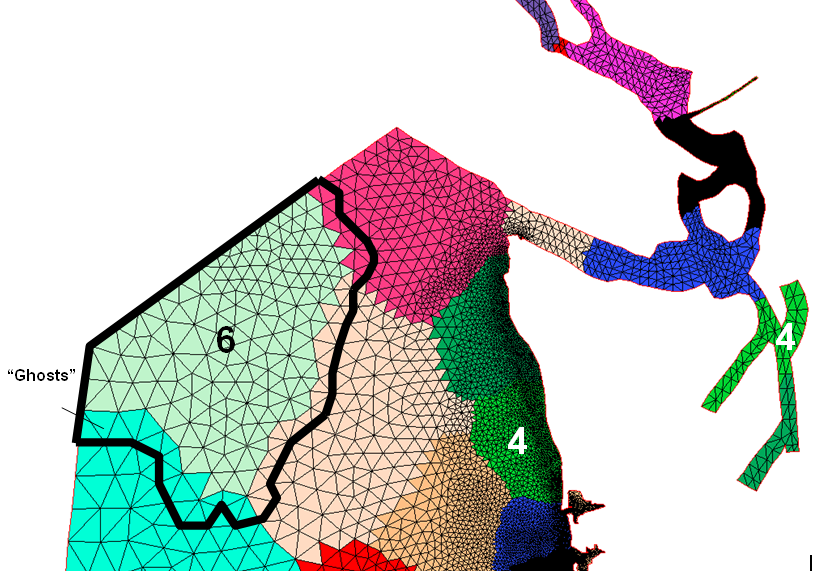
\includegraphics{FIG_wave/GRID_ParmetisB.png}}\par
\end{center}
\end{itemize}
}


\frame{
  \frametitle{Coupling of {\tt MPI} parallel programs}
\begin{itemize}
\item There are essentially two approaches to the coupling of {\tt MPI} programs:
\begin{itemize}
\item One is to use the coupled models as subroutines that are called one from the other.
\item Another is to split the set of processors considered into separate blocks. Each block of processors is assigned to a specific model.
\end{itemize}
\item We choose second solution, which is simpler. Merging two {\tt MPI} programs together takes only a few lines, we just have to change which block of processors is used.
\item The problem is to strike the right balance between number of processors for each models.
\item However, in the end the right solution may be to use the first method. But it requires to swap from one model to the next.\\
It is the solution used at {\tt ECMWF}.
\end{itemize}
}


\frame{
  \frametitle{Model coupling library, {\tt PGMCL} }
\begin{itemize}
\item The exchange between coupled models requires the sending of data between them.
\item A priori the grids are different, the model nature may be different (Structure/Unstructured grids) and so interpolation is needed between the models.
\item There are several existing libraries {\tt MCT}, {\tt OASIS}, {\tt PALM}, etc but when considering them, they appear all relatively complicated.
\item We considered {\tt MCT} and it appeared to be impossible to achieve the goals that we wanted (optimal exchanges, interpolation, performance, etc.).
\item Henceforth, we designed our own library {\tt PGMCL} (Parallel Geophysical Model Coupling Library) for coupling models.
\item After declarations, the commands become as simple as
\begin{center}
{\tt CALL MPI\_INTERP\_SEND(TheArr\_WAVtoOCN, Hwave)}\\
{\tt CALL MPI\_INTERP\_RECV(TheArr\_WAVtoOCN, Hwave)}
\end{center}

\end{itemize}
}


\begin{frame}[fragile]
  \frametitle{Multi model formalism}

Now finally we have an integrated system for coupling system:
\begin{itemize}
\item It supports the {\tt WAM} and {\tt WWM} models.
\item It has support for the {\tt ROMS} and {\tt COSMO} models.
\item The choice between model configurations is done very simply by {\tt makefile}:
\begin{verbatim}
#
# Select the models that you want to use
#
HaveWAM   ?= on
HaveWWM   ?=
HaveROMS  ?=
HaveCOSMO ?= on
\end{verbatim}

\end{itemize}
\end{frame}










\frame{
\begin{center}
\begin{tabular*}{7cm}{c}
\\[-0.5cm]
{\Huge \textcolor{blue}{III. }\textcolor{red}{Coupling}}\\[4mm]
{\Huge \textcolor{red}{of circulation}}\\[4mm]
{\Huge \textcolor{red}{and wave models}}
\end{tabular*}
\end{center}
}


\frame{
  \frametitle{The wave action equation}
\begin{itemize}
\item The wave action density satisfies the Wave Action Equation (\textcolor{red}{WAE}) which represents advection, refraction, frequency shifting and source terms:
\begin{equation*}
\frac{\partial N}{\partial t} + \nabla_x(({\bf c}_g+{\bf u}_A)N) + \nabla_k(\dot{k} N) 
 + \nabla_{\theta}(\dot{\theta} N) = S_{tot}
\end{equation*}
with
\begin{equation*}
S_{tot} = S_{in} + S_{nl3} + S_{nl4} + S_{bot} + S_{ds} + S_{break} + S_{bf}
\end{equation*}
\item The advection velocity ${\bf u}_A$ is usually approximated by ${\bf u}_{surf}$
\item The dispersion relation is changed to
\begin{equation*}
\sigma^2 = g k  \tanh( kh) \mbox{~and~} \omega = \sigma + {\bf k}\cdot {\bf u}_{A}
\end{equation*}
with $\sigma$ the intrinsic frequency and $\omega$ the absolute frequency.
\item There are more accurate expressions for ${\bf u}_A$.
\end{itemize}
}







%\frame{
%  \frametitle{The WWM model}
%The Wind Wave Model is a third generation wave model authored by Aron Roland and which shares many common features with WaveWatch III.
%\begin{itemize}
%\item The Wind Wave Model (WWM) is a unstructured grid spectral wave model.
%\item It incorporates most existing source term formulation for wind input and dissipation (Cycle III, Cycle IV, Ardhuin, Makin, ...)
%\item It has been coupled to SELFE, SHYFEM, TIMOR and ROMS.
%\item It uses Residual Distribution schemes for the horizontal advection.
%\item It integrates the WAE by using the Operator Splitting Method in explicit or implicit mode.
%\item It has NETCDF output/input/hotfile.
%\item Parallelization is done by ParMETIS.
%\end{itemize}
%}



%\frame{
%  \frametitle{The {\tt ROMS} model}
%The {\tt ROMS} model (by Hernan Arango) is a finite difference model that solves the Eulerian primitive equation in curvilinear coordinates.
%\begin{equation*}
%\frac{\partial u}{\partial t} +u\frac{\partial u}{\partial x}
%+v\frac{\partial u}{\partial y}+w\frac{\partial u}{\partial z}
%= {\bf F}
%\end{equation*}
%The {\tt ROMS} model:
%\begin{itemize}
%\item uses the hydrostatic and Boussinesq approximations,
%\item uses sigma-coordinates for the vertical discretization,
%\item uses the split-explicit method in order to resolve fast surface waves with a barotropic model,
%\item has a variety of high order schemes for momentum advection, tracer advection, horizontal pressure gradient, etc.,
%\item has infrastructure for coupling with other models
%({\tt SWAN}, {\tt WRF}, etc.),
%\item has 4DVAR assimilation capabilities (not used here),
%\item has biological and sediment sub models (not used here).
%\end{itemize}
%There are some other branches {\tt ROMS UCLA} and {\tt ROMS IRD}.
%}


\frame{
  \frametitle{Stokes drift}
\begin{itemize}
\item The time average of Eulerian velocities of waves is zero.
\item But if one considers a Lagrangian viewpoint, i.e. follows the particles then there is a movement:
\begin{center}
\resizebox{7cm}{!}{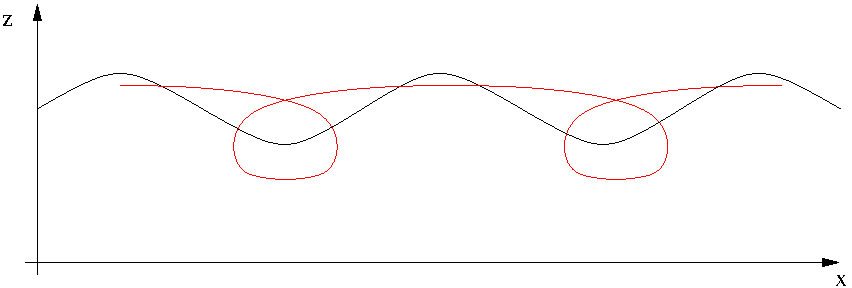
\includegraphics{FIG_wave/StokesDrift.pdf}}\par
\end{center}
\item An approximate expression of the horizontal Stokes drift $(u,v)_s$ is obtained as integral over the spectrum:
\begin{equation*}
(u,v)_{s} = \int_{\bf k} \frac{\sigma N({\bf k}) }{2\sinh^2(k(h+\xi))}\sigma {\bf k}\cosh(2k(z+h)) d{\bf k}.
\end{equation*}
%Note that the formula is actually an approximation assuming that the current shear is small.
\item For a complete description, the vertical Stokes drift is needed. It is obtained from the equation $div(u_s, v_s, w_s)=0$.
%\begin{equation*}
%\frac{\partial u_s}{\partial x} + \frac{\partial v_s}{\partial y} + \frac{\partial w_s}{\partial z} = 0
%\end{equation*}
%and so we can get $w_s$ by vertical integration from the bottom at $z=-h$ to $z=\xi$.
\end{itemize}
}




\frame{
  \frametitle{Wave coupling}

\begin{itemize}
\item Wave models use surface currents for the advection of wave energy and
the free surface enters into the dispersion relation.
\item On the other hand oceanic model can use wave information to:
\begin{itemize}
\item Compute the Stokes drift (current induced by waves, a nonlinear effect).
\item Compute the wave radiation pressure term in the primitive equation.
\item Improve the computation of the surface stress, turbulence.
\item Be used in sediment transport models.
\end{itemize}
\item Thus it makes sense to have oceanic and wave models coupled both ways. We chose to work with the {\tt ROMS} model (a finite difference model) and the {\tt WWM} model (a finite element model by Aron Roland).
\end{itemize}
\begin{center}
\resizebox{4cm}{!}{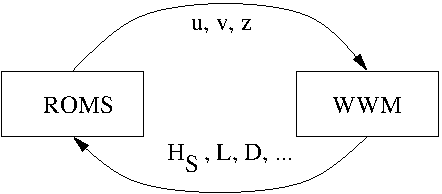
\includegraphics{FIG_wave/Model_Coupling.pdf}}\par
\end{center}
}





%\frame{
%  \frametitle{Numerics of the coupling}
%\begin{itemize}
%\item The mathematical expressions occurring in wave coupling theories are dangerous expressions like:
%\begin{equation*}
%\frac{\cosh(2k (z+h))}{\sinh(2k (h+\xi))}
%\end{equation*}
%\item This kind of function is very singular. Their large values are concentrated on the surface. On the other hand it satisfies a specific integral property:
%\begin{equation*}
%\frac{1}{h+\xi} \int_{-h}^{\xi} \frac{\cosh(2k (z+h))}{\sinh(2k (h+\xi))} dz=\frac{1}{2k(h+\xi)}
%\end{equation*}
%which has to be reproduced in the model.
%\item The solution that we choose is for every vertical cell of the model, to compute explicitly the integral and put the average value at the relevant point.
%\item We also use a $k_{eff} = \frac{1}{D} \min(300, k(h+\xi))$.
%\end{itemize}
%}






\frame{
  \frametitle{Generalized Lagrangian mean}
\begin{itemize}
\item The idea is to decompose the current as ${\bf u}_{tot} = {\bf u} + {\bf u}_{wave} + {\bf u}_{turb}$ with ${\bf u}$ the steady motion, ${\bf u}_{wave}$ the wave motion and ${\bf u}_{turb}$ the microscopic turbulent motion.
\item Under the assumption that ${\bf u}_{turb}$ is uncorrelated to other motion, we have to investigate the relation between ${\bf u}_{wave}$ and ${\bf u}$ (called \textcolor{red}{Quasi-Eulerian}).
\item We can thus introduce a new particular derivative operator
\begin{equation*}
\frac{D}{Dt} = \frac{\partial }{\partial t} + 
(u+u_{S}) \frac{\partial }{\partial x} +
(v+v_{S}) \frac{\partial }{\partial y} +
(w+w_{S}) \frac{\partial }{\partial z}
\end{equation*}
and the equation for tracers $T$ (i.e. salinity, temperature, turbulent kinetic energy, etc.) is then
\begin{equation*}
\frac{D T}{Dt} = S_{source/sink}(T) + S_{diffusion}(T)
\end{equation*}
%with $C(T)$ the source and sink term and $D(T)$ the diffusion term.
\item Complete primitive equations by Bennis/Ardhuin 2011 are more complicated.
\end{itemize}
}






\frame{
  \frametitle{Exchange between Stokes current and current}

\begin{center}
\begin{minipage}{4.6cm}
\centering
\epsfig{file=NCLpictures_drifter/DoNCL_Bennis/Bennis_a_HsB.eps, height=4.2cm}\par
%\resizebox{5.4cm}{!}{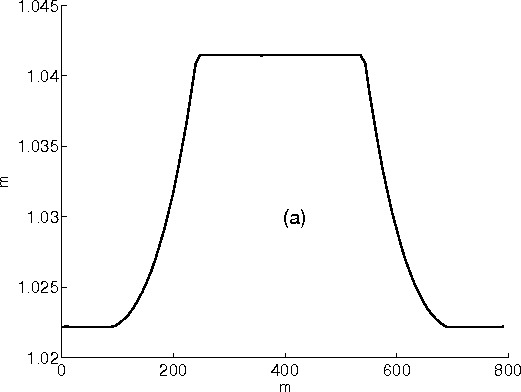
\includegraphics{DrifterPicture/Bennis_second_test/Hwave/Hsignificant18000.jpg}}\par
\end{minipage}
\begin{minipage}{4.6cm}
\centering
\epsfig{file=NCLpictures_drifter/DoNCL_Bennis/Bennis_b_TotalLagB.eps, height=4.2cm}\par
%\resizebox{5.4cm}{!}{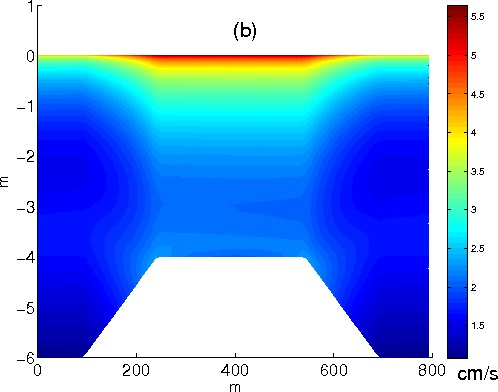
\includegraphics{DrifterPicture/Bennis_second_test/UVlag/Vmagnitude_w18000.jpg}}\par
\end{minipage}
\begin{minipage}{4.6cm}
\begin{itemize}
\item The stokes drift flux is not conservative
\item But the flux $(h+ \xi)(\overline{u} + \overline{u}_s)$ is constant in that test case.
\end{itemize}
\end{minipage}
\begin{minipage}{4.6cm}
\centering
\epsfig{file=NCLpictures_drifter/DoNCL_Bennis/Bennis_c_CurrB.eps, height=4.2cm}\par
%\resizebox{5.4cm}{!}{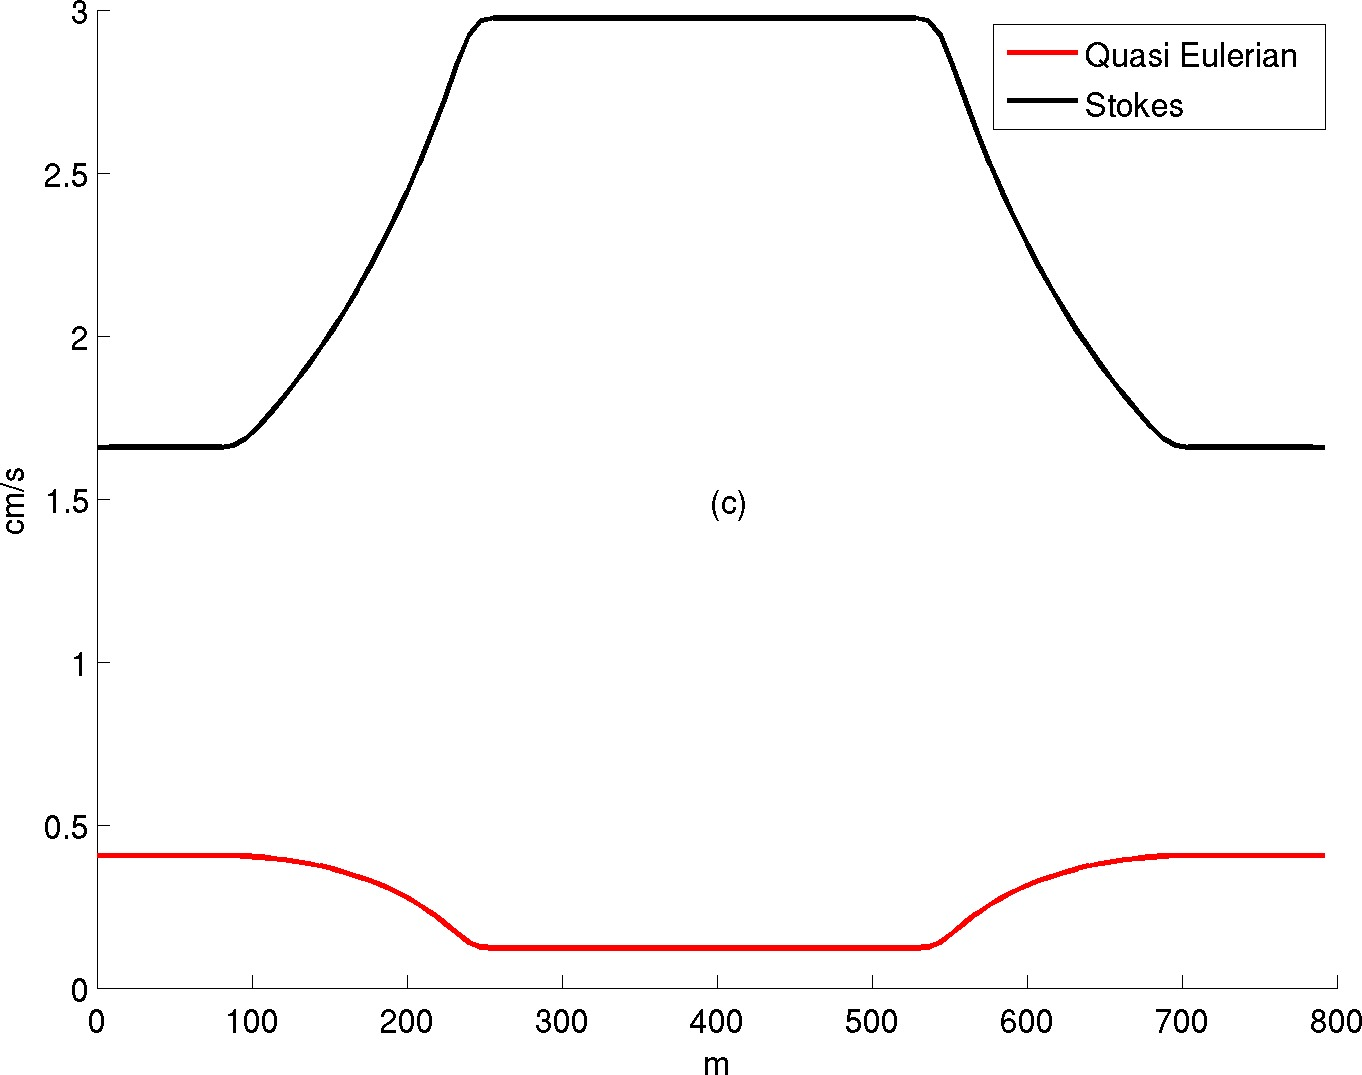
\includegraphics{DrifterPicture/Bennis_second_test/UVbarLag/BaroU_Us18000.jpg}}\par
\end{minipage}
\end{center}
}












\frame{
  \frametitle{Bathymetry and rivers of the Adriatic Sea}
\begin{itemize}
\item The bathymetry varies a lot from 1200m to 50m.
\item The island structure on the Croatian side is quite complex.
\item River inflow is more important than in other parts of the Mediterranean.
\end{itemize}

\begin{center}
\begin{minipage}[b]{5.3cm}
%l b r t
\resizebox{5.2cm}{!}{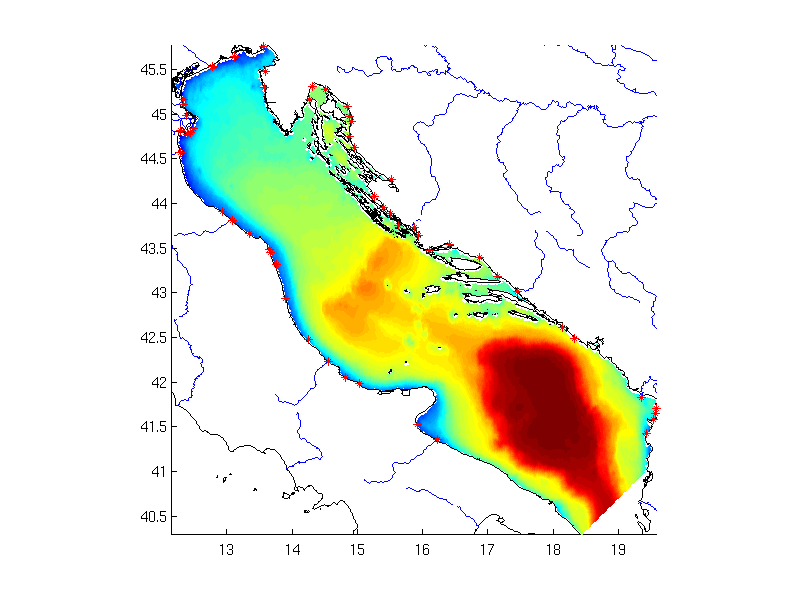
\includegraphics[trim=35mm 11mm 35mm 11mm, clip]{PictureElect/BathymetryRiver.png}}\par
%\resizebox{5.5cm}{!}{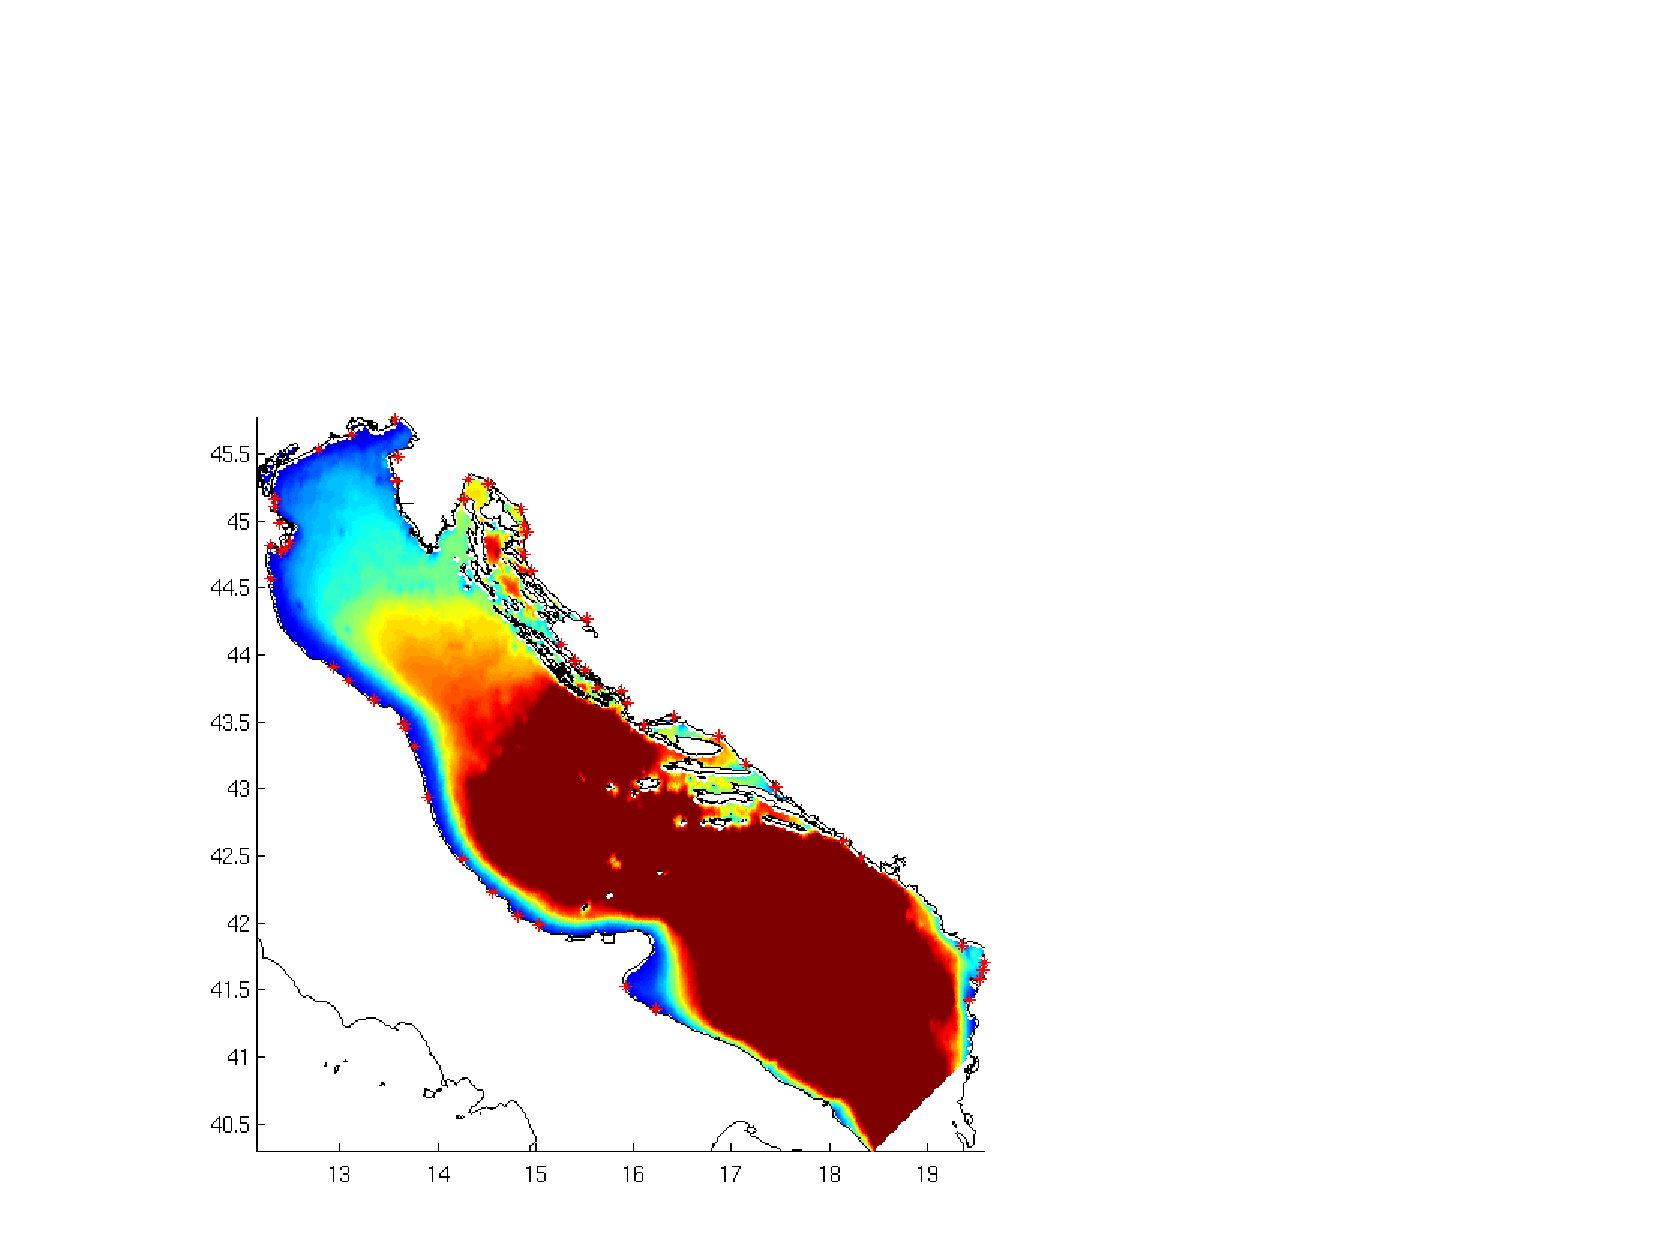
\includegraphics[bb=101 32 477 403, clip]{PictureElect/BathymetryRiver_V1.pdf}}\par
\end{minipage}
\begin{minipage}[b]{5.3cm}
\begin{itemize}
\item Significant inflow/outflow occurs at the Ottranto strait and generates the highest tides of the Mediterranean.
\item Two winds bora and sirocco dominate the general circulation.
\end{itemize}
\end{minipage}
\end{center}
}

%\frame{
%  \frametitle{Chosen forcing information}
%\begin{itemize}
%\item The chosen modelization of the Adriatic Sea uses the atmospheric forcing fields from {\tt DHMZ} using the {\tt ALADIN} model (sea surface pressure, temperature, humidity, rain, cloud factor, short wave radiation).
%\item For river forcing, we used:
%\begin{itemize}
%\item Hourly measurements for Po river and Neretva river.
%\item Daily flux measurements for 9 other rivers and temperature for 5 more.
%\item For other Italian rivers, we used climatological information from Raicich, 1994. For other Croatian rivers we rescale according to Neretva inflow.
%\item For temperature we took nearest river.
%\end{itemize}
%\item We used an initial state obtained from {\tt AREG} which is an operational model using a modification of {\tt POM}.
%\item At the open boundary of the Ottranto strait, we used daily average from the {\tt AREG} model and we add tidal signal to it.
%\end{itemize}
%}




\frame{
  \frametitle{Bora event I}
\begin{center}
\begin{minipage}{5.3cm}
\centering
\resizebox{5.5cm}{!}{\includegraphics{NCLpictures_buoy/DoNCL_BoraTime/TheWindB.eps}}\par
\end{minipage}
\begin{minipage}{5.3cm}
\centering
\resizebox{5.5cm}{!}{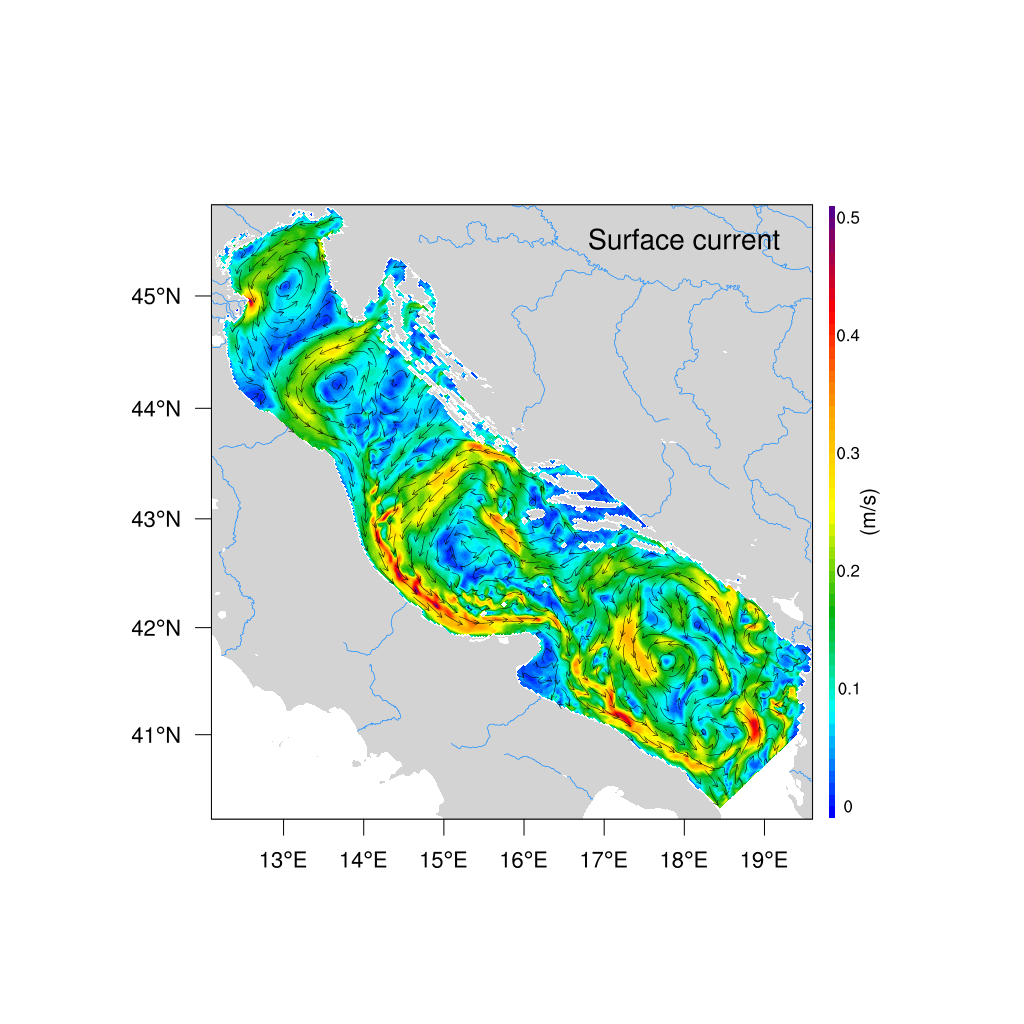
\includegraphics{NCLpictures_buoy/DoNCL_BoraTime/TheCurrentB.eps}}\par
\end{minipage}
\end{center}

\begin{itemize}
\item Wind speed and surface current at 2007-11-17 06:00:00 during a bora event.
\item The bora jets induce a multiple gyre structure on surface currents.
\end{itemize}

}




\frame{
  \frametitle{Bora event II}
\begin{center}
\begin{minipage}{5.3cm}
\centering
\resizebox{5.5cm}{!}{\includegraphics{NCLpictures_buoy/DoNCL_BoraTime/HwaveB.eps}}\par
\end{minipage}
\begin{minipage}{5.3cm}
\centering
\resizebox{5.5cm}{!}{\includegraphics{NCLpictures_buoy/DoNCL_BoraTime/DiffHwaveB.eps}}\par
\end{minipage}
\end{center}

\begin{itemize}
\item Coupling led to a decrease of $H_s$ in the bora jet and an increase outside of the jet due to opposing currents.
\end{itemize}
Work done in collaboration with M. Kuzmi\'c (IRB), I. Janekovi\'c (IRB), I. Toma\u zi\'c (ESA) and A. Roland (TU Darmstadt)
}



\frame{
  \frametitle{Impact on surface currents}

\begin{itemize}
\item The most significant impact of coupling with wave model on surface currents is the parameterization $z_{0,sea} = 0.5 H_s$ of sea roughness length.
\begin{itemize}
\item Reduction of $15$ cm/s of current speed during bora events on the tip of Istria
\end{itemize}
\item The next most significant effect is the effect of GLM formulation with reduction of current speed by $3$ cm/s on the Italian coastline
\item Finally the use of surface stress from the wave model is difficult to assess but leads to further decrease of surface currents in the bora jet.
\end{itemize}
}





\frame{
\begin{center}
\begin{tabular*}{7cm}{c}
\\[-0.5cm]
{\Huge \textcolor{blue}{IV. }\textcolor{red}{Coupling}}\\[4mm]
{\Huge \textcolor{red}{of atmosphere}}\\[4mm]
{\Huge \textcolor{red}{and wave models}}
\end{tabular*}
\end{center}
}



%\frame{
%  \frametitle{Stochastic wave modelling}
%\begin{itemize}
%\item Oceanic models are using grids (structured or unstructured) of size $1km\leq d\leq 10km$ to simulate the ocean
%\item But oceanic waves have a typical wavelength $2m$ $\leq$ $L$ $\leq$ $100m$. So, we cannot resolve waves in the ocean.
%\item But if one uses phase averaged models and uses stochastic assumptions then it is possible to model waves by a spectral wave action density $N({\bf x},{\bf k})$
%\item This density satisfies a Wave Action Equation (\textcolor{red}{WAE}) which represents advection, refraction, frequency shifting and source terms:
%\begin{equation*}
%\frac{\partial N}{\partial t} + \nabla_x(({\bf c}_g+{\bf u}_A)N) + \nabla_k(\dot{k} N) 
% + \nabla_{\theta}(\dot{\theta} N) = S_{tot}
%\end{equation*}
%with
%\begin{equation*}
%S_{tot} = S_{in} + S_{nl3} + S_{nl4} + S_{bot} + S_{ds} + S_{break} + S_{bf}
%\end{equation*}
%\end{itemize}
%}




%\frame{
%  \frametitle{Doppler shift}
%\begin{itemize}
%\item Suppose that we have a uniform current ${\bf u}$ then the dispersion relation is changed to
%\begin{equation*}
%\sigma^2 = g k  \tanh( kh) \mbox{~and~} \omega = \sigma + {\bf k}\cdot {\bf u}
%\end{equation*}
%with $\sigma$ the intrinsic frequency and $\omega$ the absolute frequency.
%\item In the case of a sheared current, the Doppler shift relation changes to
%\begin{equation*}
%\omega = \sigma + {\bf k}\cdot\int_{z=-h}^{z=\xi} {\bf u} \frac{2k\cosh(2k(z+h))}{\sinh(2kD)} dz
%\end{equation*}
%\item The advection velocity ${\bf u}_A$ is usually approximated by the surface current velocity. There is unfortunately no Wave Action Equation in the case of sheared currents.
%\end{itemize}
%}







\frame{
  \frametitle{Surface stress}
\begin{itemize}
\item Surface stress is a key unknown in many oceanographic simulations.
\item It is expressed as $\tau = \rho_{air} u^2_*$ with $u_*$ being the friction velocity.
\item We have the following expression for the wind near the sea surface:
\begin{equation*}
U(z) = \frac{u_*}{\kappa} \left\lbrack \ln \left(\frac{z}{z_{0,air}}\right) + \psi(z, z_0, L)\right\rbrack
\end{equation*}
with
\begin{itemize}
\item $z_{0,air}$ the air roughness length
\item $\psi$ the stability correction and $L$ the Monin-Obukhov length
\item $\kappa$ is the von-Karman constant (around $0.41$)
\end{itemize}
\item To get a solvable system, we need one more equation for 
\begin{equation*}
\alpha = z_{0,air} \frac{g}{u_{*}^2}
\end{equation*}
which is called the Charnock coefficient (nondimensional).
\item Many empirical formulas for $\alpha$ depending on the wind speed $U(10m)$ have been proposed.
\end{itemize}
}





%\frame{
%  \frametitle{Comparison with QuikSCAT of ALADIN windspeed}
%\begin{center}
%\begin{minipage}{5.3cm}
%\centering
%\resizebox{5.5cm}{!}{\includegraphics{NCLpictures_buoy/DoNCL_ScatterQS/MagScatter.eps}}\par
%\end{minipage}
%\end{center}
%\begin{itemize}
%\item Wind speed is systematically underestimated by atmospheric models.
%\item Reasons seems to be too small resolution and less sophisticated model than {\tt IFS}.
%\item Problems in direction as well.
%\end{itemize}
%}





\frame{
  \frametitle{Comparison of Charnock coefficient}
\begin{center}
\begin{minipage}{5.3cm}
\centering
\resizebox{5.5cm}{!}{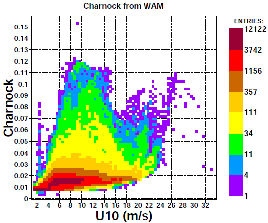
\includegraphics{FIG_wave/WAM_Charnock.png}}\par
\end{minipage}
\begin{minipage}{5.3cm}
\centering
\resizebox{5.5cm}{!}{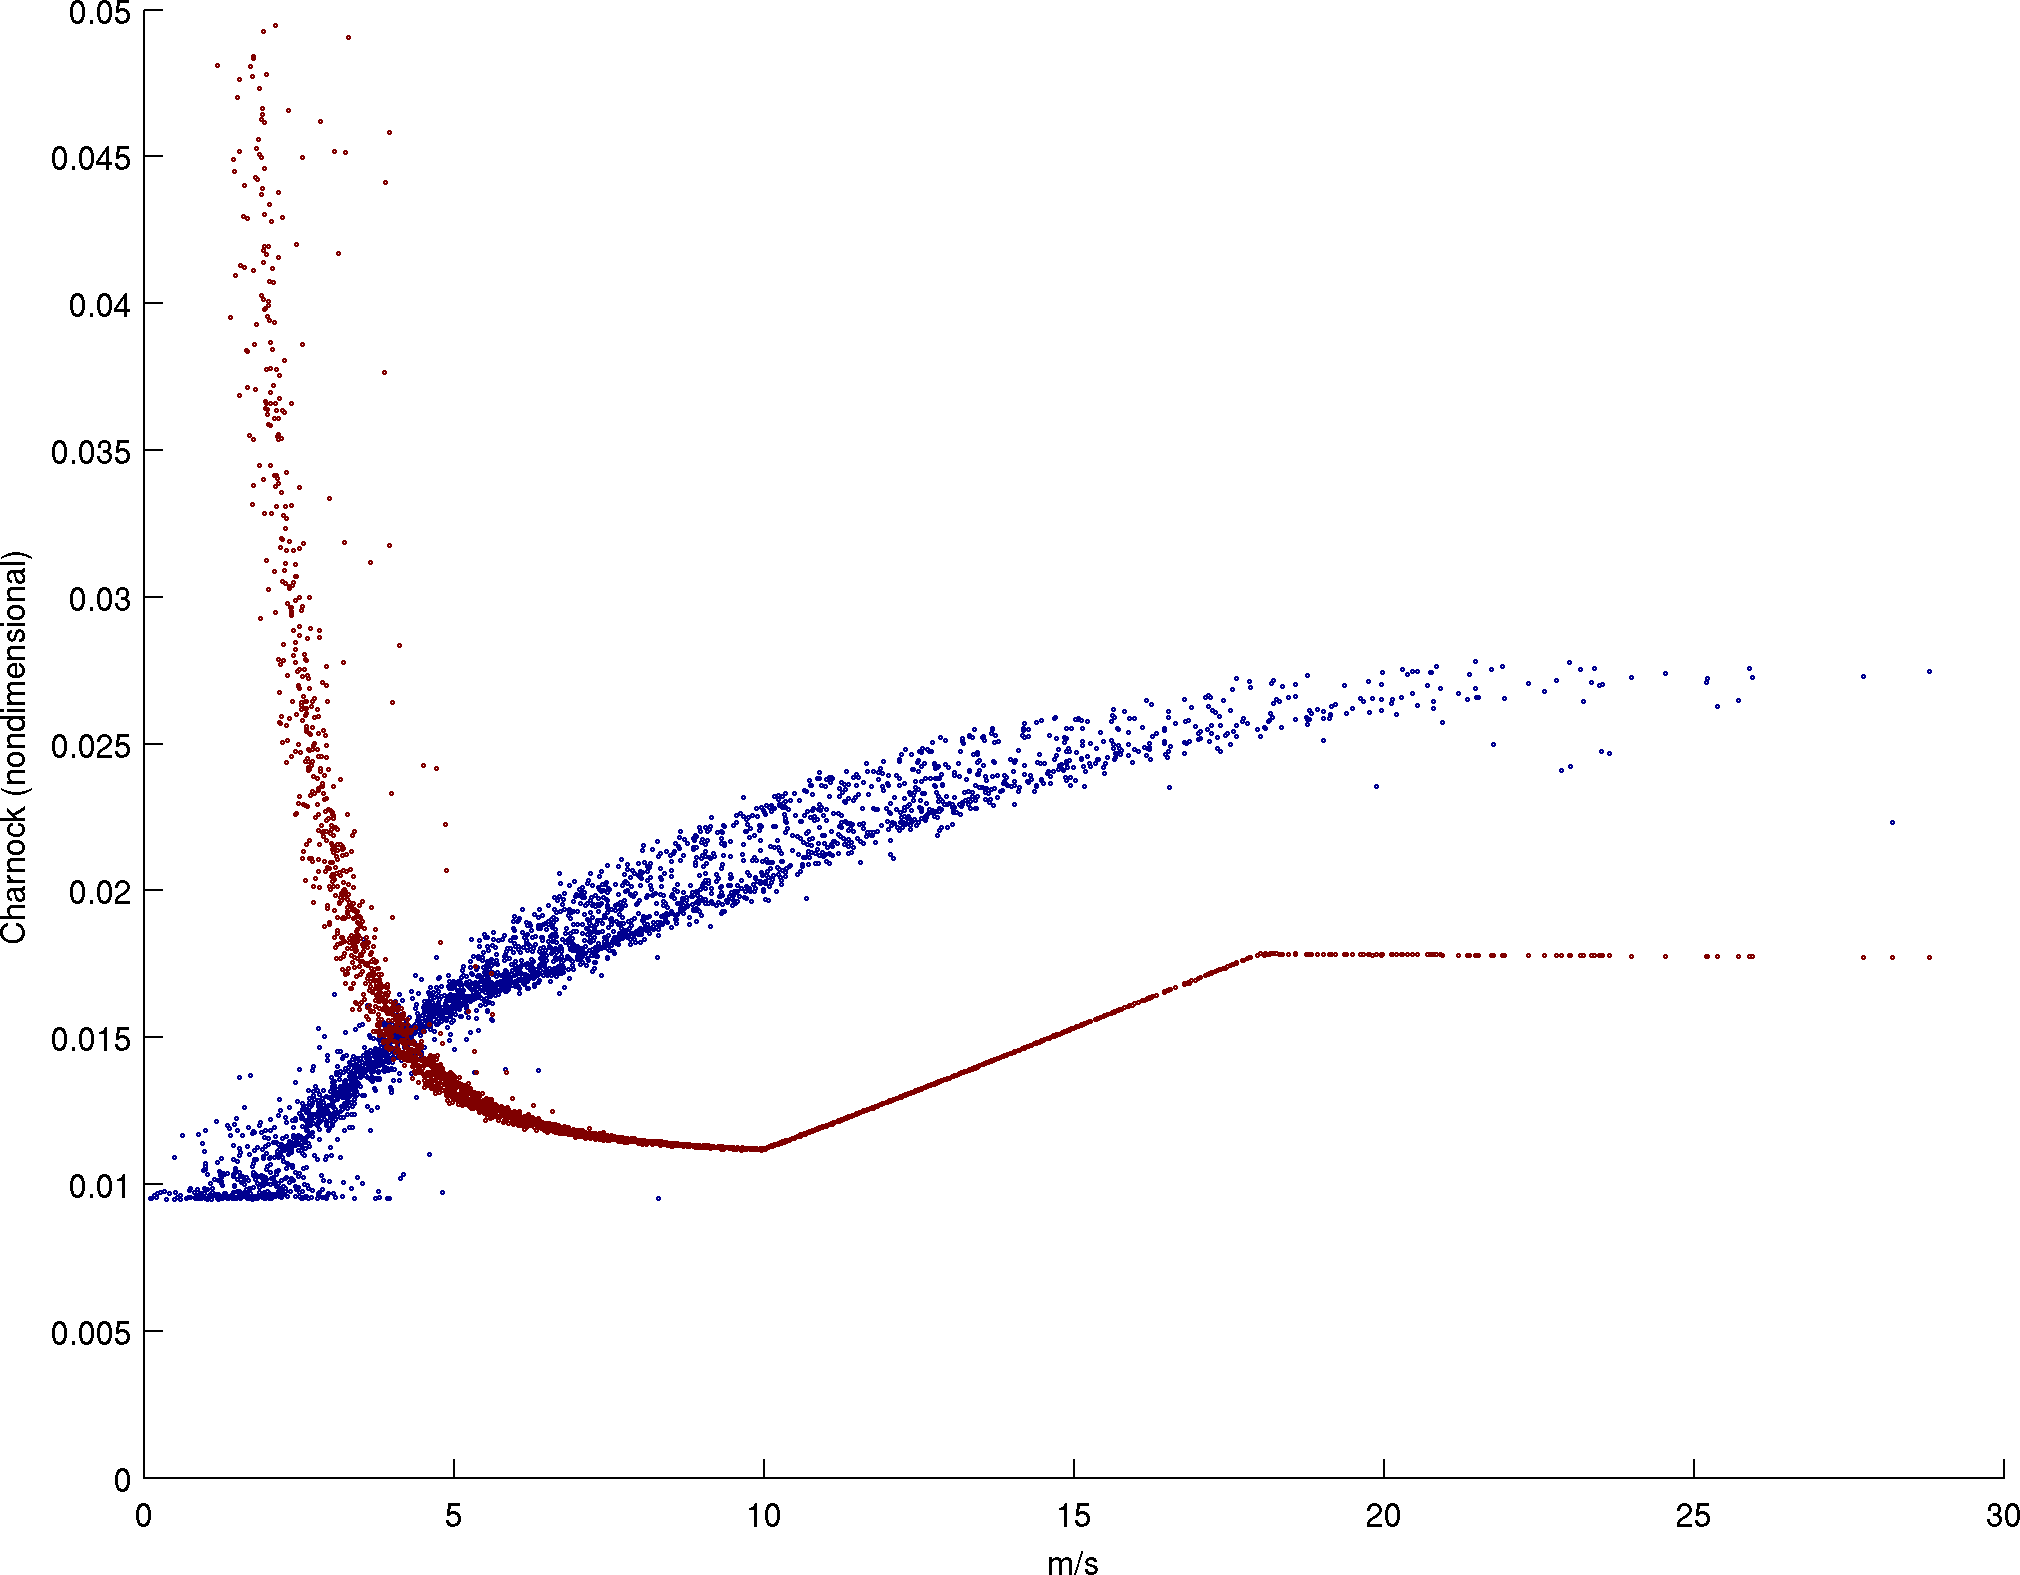
\includegraphics{DrifterPicture/Scatter_Charnock/Scatter_bulk_wave.png}}\par
\end{minipage}
\end{center}

\begin{itemize}
\item There are large variability of Charnock expressed in function of the wind.
\item A priori, the wave model has a good idea of the roughness of the sea and so it makes sense to use the Charnock coefficient computed from the wave model.
\end{itemize}
}

\frame{
  \frametitle{Peter Janssen formulation}
\begin{itemize}
\item Janssen (1989) proposed to decompose the stress into
\begin{equation*}
\tau = \tau_{viscous}  + \tau_{wave} + \tau_{high.\,freq.}
\end{equation*}
\item The term $\tau_{viscous}$ is negligible for sea applications.
\item Janssen (1989) proposed a parameterization of the high frequency stress
\item And $\tau_{wave}$ is obtained as an integral over the wind input formula of the wave model.
\item Then the idea is to compute the Charnock coefficient in the wave model and send it to the atmospheric model.
\item This coupling strategy is implemented in {\tt ECMWF} since 1998 and results in improved forecasts results.
\end{itemize}
}

\frame{
  \frametitle{Coupling of {\tt WAM} and {\tt COSMO}}
\begin{itemize}
\item Both models were coupled with the {\tt PGMCL}.
\item We follow the same strategy as the one between {\tt IFS} and {\tt WAM}.
\begin{center}
\resizebox{4cm}{!}{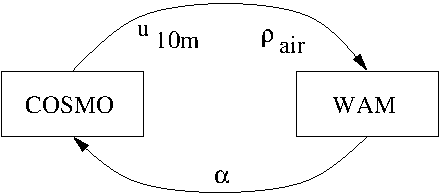
\includegraphics{FIG_wave/Model_CouplingWAM_COSMO.pdf}}\par
\end{center}
\item We run the model over a period of two months over the Mediterranean Sea for Nov. Dec. 2010
\begin{center}
\resizebox{4cm}{!}{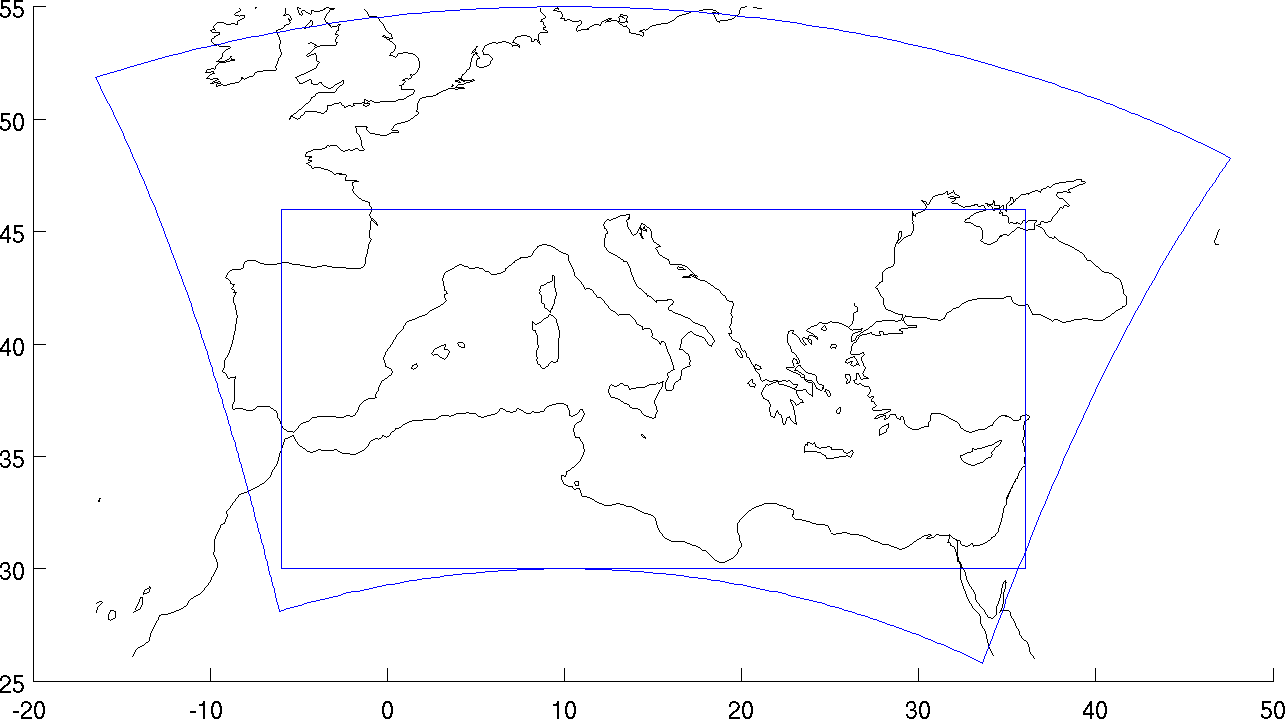
\includegraphics{FIG_wave/MapSimulation.png}}\par
\end{center}
\end{itemize}
Work done in collaboration with P. Janssen/J. Bidlot ({\tt ECMWF}), L. Cavaleri ({\tt ISMAR}), L. Torrisi ({\tt CNMCA}, Italian Nat. Met. Center) and A. Roland (TU Darmstadt)
}


\frame{
  \frametitle{Results}
ME: Mean Error \mbox{~~~~} RMSE: Root Mean Square Error
\begin{itemize}
\item For comparison of wave height with all buoys we get:
\begin{center}
\begin{tabular}{|c|c|c|}
\hline
         & ME     & RMSE\\
\hline
Coupled     & 0.11 m & 0.55 m\\
Uncoupled   & 0.21 m & 0.62 m\\
\hline
\end{tabular}
\end{center}
\item For comparison of wave height with Envisat altimeter satellite we get:
\begin{center}
\begin{tabular}{|c|c|c|}
\hline
         & ME    & RMSE\\
\hline
Coupled     & 0.25 m  & 0.65 m\\
Uncoupled   & 0.43 m  & 0.85 m\\
\hline
\end{tabular}
\end{center}
\item For comparison of wind speed at $10$m with Envisat altimeter satellite we get:
\begin{center}
\begin{tabular}{|c|c|c|}
\hline
         & ME       & RMSE\\
\hline
Coupled     & 0.25 m/s & 2.28 m/s\\
Uncoupled   & 0.44 m/s & 2.44 m/s\\
\hline
\end{tabular}
\end{center}




\end{itemize}
}







%\frame{
%  \frametitle{Grids of the Adriatic}
%trim=l b r t
%\begin{center}
%\begin{minipage}{5.2cm}
%\resizebox{5.2cm}{!}{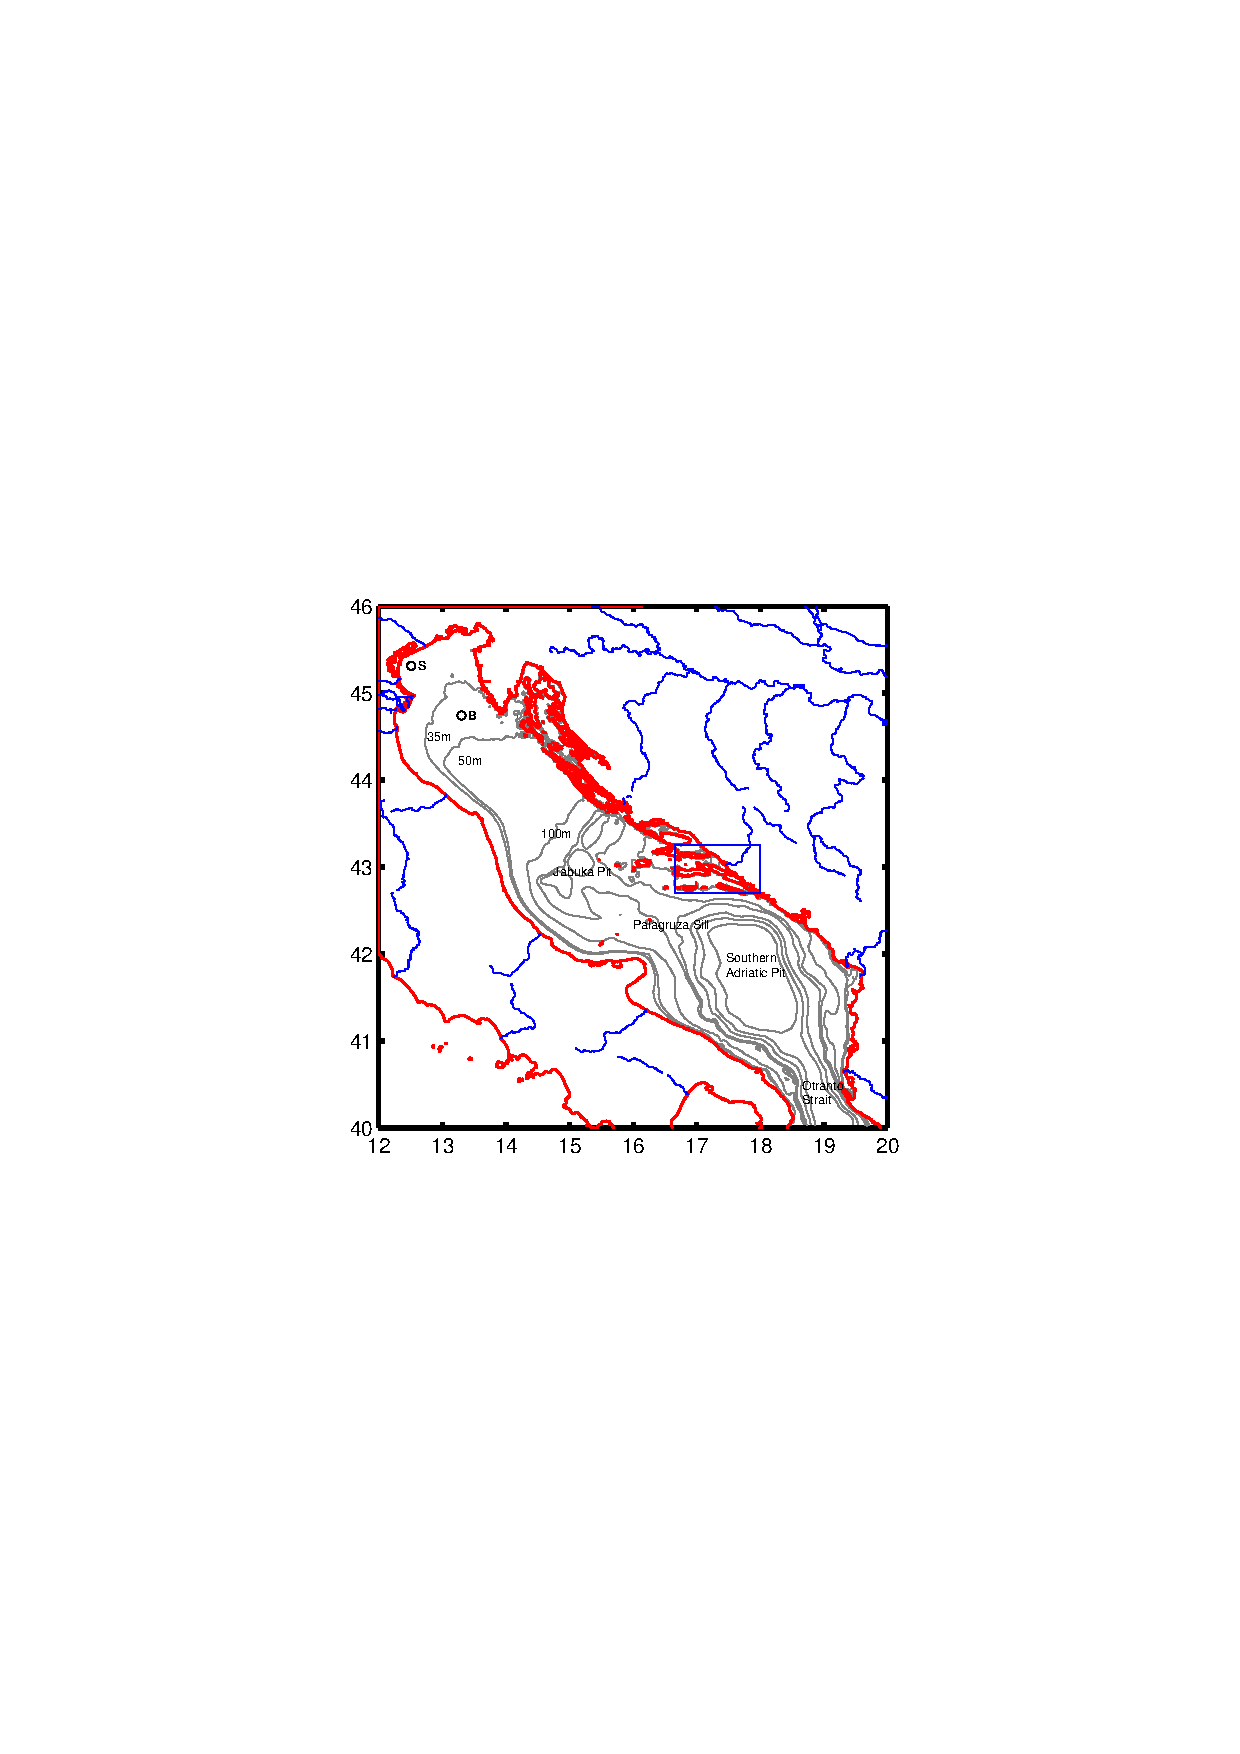
\includegraphics[bb=166 390 399 555,clip]{FIG_wave/Stations300_AASSb.pdf}}\par
%\end{minipage}
%\begin{minipage}{5.2cm}
%\resizebox{6.3cm}{!}{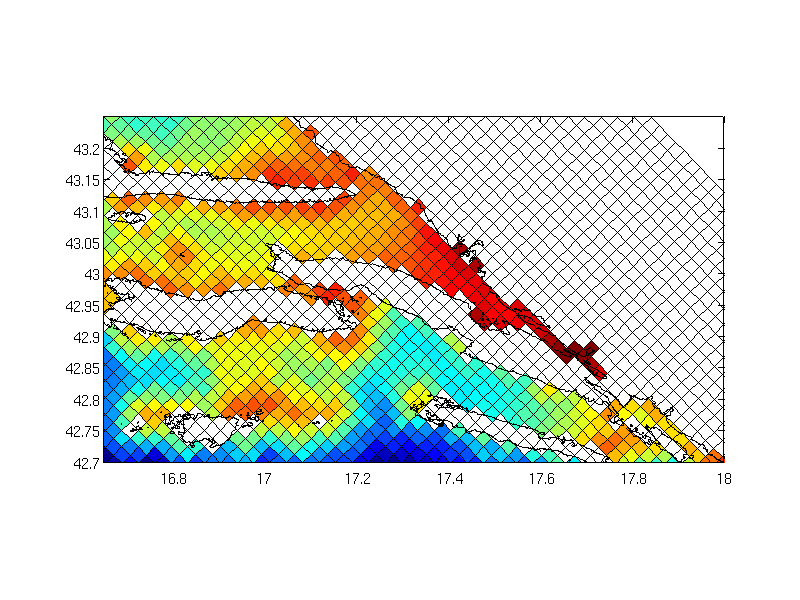
\includegraphics[trim=16mm 28mm 16mm 28mm, clip]{FIG_wave/PicCompar/RomsGrid.png}}\par
%\end{minipage}
%\end{center}
%\begin{center}
%\begin{minipage}{5.2cm}
%\resizebox{5.8cm}{!}{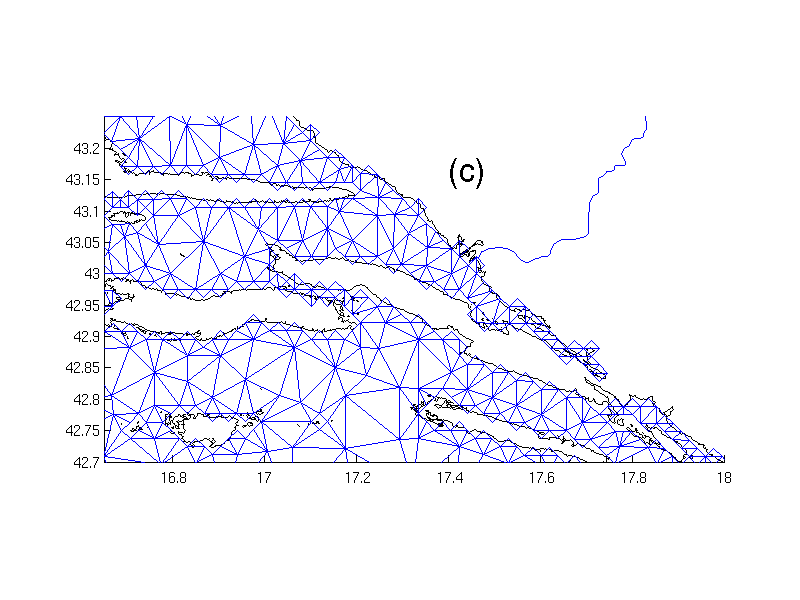
\includegraphics[trim=16mm 28mm 16mm 28mm, clip]{FIG_wave/PicCompar/FEMgrid1.png}}\par
%\end{minipage}
%\begin{minipage}{5.2cm}
%\resizebox{5.8cm}{!}{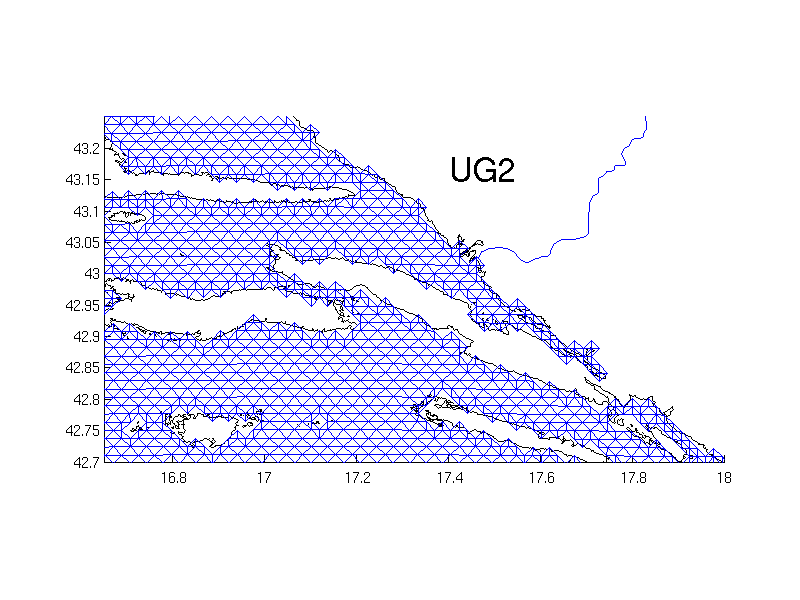
\includegraphics[trim=16mm 28mm 16mm 28mm, clip]{FIG_wave/PicCompar/FEMgrid2.png}}\par
%\end{minipage}
%\end{center}
%}





%\frame{
%  \frametitle{Possible extensions}
%\begin{itemize}
%\item We did the coupling of COSMO and WAM. Key point is the Charnock coefficient is computed in the WAM model and used by the atmospheric model.
%\begin{itemize}
%\item The atmospheric model provides the wind and air density to wave model.
%\item The wave model provides the Charnock coefficient to the atmospheric model.
%\end{itemize}
%\item Results on the Mediterranean indicate a slight decrease of wind magnitude and an overall improvements in wave and wind statistics when comparing with altimeter and stations.
%\item Further coupling with Atmospheric local model, for example COSMO or WRF.
%\item Key issue is the physical parameterization of the sea surface.
%\end{itemize}
%}





\frame{
  \frametitle{}
\vspace{1.5cm}
\begin{center}
{\Huge \textcolor{red}{T}\textcolor{blue}{H}\textcolor{green}{A}\textcolor{blue}{N}\textcolor{red}{K}}\\[1cm]
{\Huge \textcolor{red}{Y}\textcolor{blue}{O}\textcolor{red}{U}}
%\epsfig{file=plit-gal10.eps, height=5.5cm}
\end{center}
}




\end{document}
